%%%%%%%%%%%%%%%%%%%%%%%%%%%%%%%%%%%%%%%%%%%%%%%%%%%%%%%%%%%%%%%%%%%%%%%%%%%%%%%%%%
\begin{frame}[fragile]\frametitle{}
\begin{center}
{\Large Vectors}
\end{center}
\end{frame}


%%%%%%%%%%%%%%%%%%%%%%%%%%%%%%%%%%%%%%%%%%%%%%%%%%%%%%%%%%%
 \begin{frame}[fragile] \frametitle{Vectors}

\begin{itemize}

\item At its simplest, a vector is an entity that has both magnitude and direction. 
\item The magnitude represents a distance (for example, ``2 miles'') and the direction indicates which way the vector is headed (for example,``East''). 
\item One more way is $\bar{v} = 2\hat{i} + 3\hat{j}$; meaning?
\item Is Magnitude-Direction form equivalent to i-j form?
\item Inter-convertible? How?
\item Can it have just two components?
\end{itemize}

\end{frame}




%%%%%%%%%%%%%%%%%%%%%%%%%%%%%%%%%%%%%%%%%%%%%%%%%%%%%%%%%%%
 \begin{frame}[fragile] \frametitle{Vectors}
Two-dimensional example:
\begin{itemize}

\item A vector that is defined by a point in a two-dimensional plane
\item A two dimensional coordinate consists of an x and a y value, and in this case we'll use 2 for x and 1 for y
\item Its is written in matrix form as : $\vec{v} = \begin{bmatrix}2 \\ 1 \end{bmatrix}$
\item Describes the movements required to get to the end point (of head) of the vector 
\item So, it is not a point in space. It gives Direction, like a movement recipe. 
\item When added to a point, results into a transformed point.
\item In this case, we need to move 2 units in the x dimension, and 1 unit in the y dimension
\end{itemize}

\end{frame}

%%%%%%%%%%%%%%%%%%%%%%%%%%%%%%%%%%%%%%%%%%%%%%%%%%%%%%%%%%%
 \begin{frame}[fragile] \frametitle{Vectors}
Two-dimensional example:
\begin{itemize}

\item Note that we don't specify a starting point for the vector
\item We're simply describing a destination coordinate that encapsulate the magnitude and direction of the vector. 
\item Think about it as the directions you need to follow to get to {\bf there} from {\bf here}, without specifying where {\bf here} actually is!
\item Generally using the point 0,0 as the starting point (or origin). Also called as Position Vector.
\item Our vector of (2,1) is shown as an arrow that starts at 0,0 and moves 2 units along the x axis (to the right) and 1 unit along the y axis (up).
\end{itemize}

\end{frame}

%%%%%%%%%%%%%%%%%%%%%%%%%%%%%%%%%%%%%%%%%%%%%%%%%%%%%%%%%%%
 \begin{frame}[fragile] \frametitle{Vectors}
Calculating Magnitude
\begin{itemize}

\item $\|\vec{v}\| = \sqrt{v_{1}\;^{2} + v_{2}\;^{2}}$
\item Double-bars are often used to avoid confusion with absolute values. 
\item Note that the components of the vector are indicated by subscript indices $(v_1, v_2,\ldots v_n)$
\item In this case, the vector v has two components with values 2 and 1, so our magnitude calculation is:
\item $\|\vec{v}\| = \sqrt{2^{2} + 1^{2}} = \sqrt{5} \approx 2.24$
\end{itemize}

\end{frame}


%%%%%%%%%%%%%%%%%%%%%%%%%%%%%%%%%%%%%%%%%%%%%%%%%%%%%%%%%%%
 \begin{frame}[fragile] \frametitle{Vectors}
Calculating Direction
\begin{itemize}

\item We can get the angle of the vector by calculating the inverse tangent; sometimes known as the arctan
\item For our v vector (2,1):$tan(\theta) = \frac{1}{2}$
\item $\theta = tan^{-1} (0.5) \approx 26.57^{o}$
\item use the following rules:
\begin{itemize}

\item Both x and y are positive: Use the tan-1 value.
\item x is negative, y is positive: Add 180 to the tan-1 value.
\item Both x and y are negative: Add 180 to the tan-1 value.
\item x is positive, y is negative: Add 360 to the tan-1 value.
\end{itemize}
\end{itemize}


\end{frame}




%%%%%%%%%%%%%%%%%%%%%%%%%%%%%%%%%%%%%%%%%%%%%%%%%%%%%%%%%%%
 \begin{frame}[fragile] \frametitle{Vectors}

\begin{itemize}

\item Vectors are defined by an n-dimensional coordinate that describe a point in space that can be connected by a line from an arbitrary origin.
\item Are n-dimensional Points and Vectors equivalent? How?
\item $\|\vec{v}\| = \sqrt{v_{1}\;^{2} + v_{2}\;^{2} ... + v_{n}\;^{2}}$
\end{itemize}

\end{frame}



%%%%%%%%%%%%%%%%%%%%%%%%%%%%%%%%%%%%%%%%%%%%%%%%%%%%%%%%%%%
  \begin{frame}[fragile]
\textbf{Definition}
  A {\em vector} is a matrix with one column.


 \textbf{Example}
  \[
  \left[\begin{array}{r}
   1 \\2 \\-5\\ 9  
  \end{array}\right]
 \]
  
  
\textbf{Note}
Two vectors are equal precisely when they have the same number
of rows and all their corresponding entries are  equal.

\end{frame}

%%%%%%%%%%%%%%%%%%%%%%%%%%%%%%%%%%%%%%%%%%%%%%%%%%%%%%%%%%%%%%%%%%%%%%%%
\begin{frame}[fragile]\frametitle{Vectors (Recap)}
\begin{itemize}
\item A vector has magnitude (how long it is) and direction
\item A point can be a vector (position vector, from Origin)
\item A data row is a point in n-dimensions, thus a vector as well.
\end{itemize}
\begin{center}
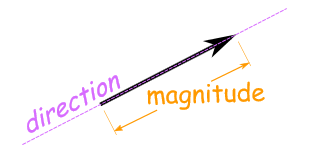
\includegraphics[width=0.5\linewidth]{vec}
\end{center}
\end{frame}

%%%%%%%%%%%%%%%%%%%%%%%%%%%%%%%%%%%%%%%%%%%%%%%%%%%%%%%%%%%
 \begin{frame}[fragile] \frametitle{Vector Addition}

\begin{center}
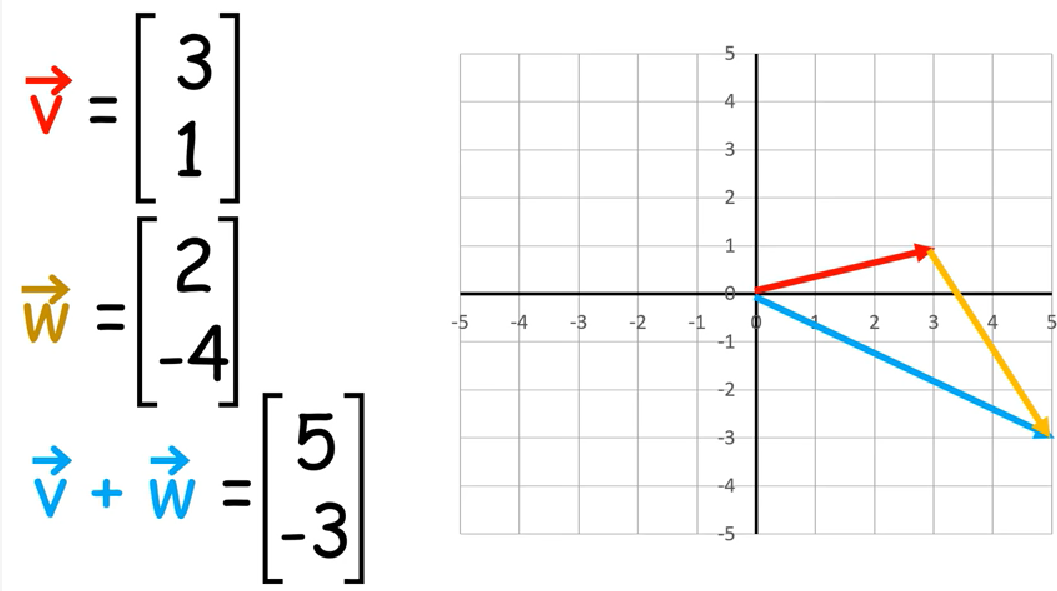
\includegraphics[width=0.5\linewidth,keepaspectratio]{vec1}
\end{center}

\begin{itemize}
\item To add these vectors: We just add the individual components, so 3 plus 2
is 5; and 1 plus -4 is -3.
\item It is simply adding another leg to the journey; so if
we follow vector V along 3 and up 1, and then follow vector W along 2 and down 4,
we end up at the head of the vector we calculated by adding V and
W together.
\end{itemize}

\end{frame}


%%%%%%%%%%%%%%%%%%%%%%%%%%%%%%%%%%%%%%%%%%%%%%%%%%%%%%%%%%%
  \begin{frame}[fragile]{Vector Addition}
 \textbf{Definition}
    We define the sum and  of two vectors by 
     \[
      \left[\begin{array}{r}
       u_1 \\ u_2 \\ \vdots \\ u_n
      \end{array}\right]
    +
    \left[\begin{array}{r}
       v_1 \\ v_2 \\ \vdots \\ v_n
      \end{array}\right]
     = 
     \left[\begin{array}{r}
       u_1 + v_1  \\ u_2 + v_2 \\ \vdots \\ u_n + v_n
      \end{array}\right]
    \]     
    and the product of a scalar and a vector by
    \[
     \alpha \left[\begin{array}{r}
       u_1 \\ u_2 \\ \vdots \\ u_n
      \end{array}\right]
    =  
    \left[\begin{array}{r}
       \alpha u_1 \\ \alpha u_2 \\ \vdots \\ \alpha u_n
      \end{array}\right]
    \]
 
\end{frame}

%%%%%%%%%%%%%%%%%%%%%%%%%%%%%%%%%%%%%%%%%%%%%%%%%%%%%%%%%%%
\begin{frame}[fragile]\frametitle{Example}

  \[
  \left[\begin{array}{r}
   1 \\ 3 \\ -5
  \end{array}\right]
+
\left[\begin{array}{r}
   2 \\ 2 \\ 7
  \end{array}\right]
 =   
 \left[\begin{array}{r}
    3 \\ 5 \\ 2 
  \end{array}\right]   
  \qquad 
  \mbox{ and } \qquad  
   3 \left[\begin{array}{r}
   5 \\ 2 \\ 1
  \end{array}\right]
=  
\left[\begin{array}{r} 15 \\ 6 \\ 3  \end{array}\right]
\]
  
\end{frame}


%%%%%%%%%%%%%%%%%%%%%%%%%%%%%%%%%%%%%%%%%%%%%%%%%%%%%%%%%%%
\begin{frame}[fragile]\frametitle{Exercise}

Let $\vec{u}$ and $\vec{v}$ be given by 
\[
 \vec{u} = \left[\begin{array}{r} 1 \\ 1 \end{array}\right]
 \qquad \mbox{and} \qquad
 \vec{v} = \left[\begin{array}{r} 1 \\ -1 \end{array}\right]
\]
Plot  $\vec{u}$, $\vec{v}$, $\vec{2u}$ and 
$\vec{u}+\vec{v}$.


\textbf{Parallelogram rule for vector addition}
Suppose $\vec{u}$ and $\vec{v}\in \mathbb R^2$.  Then 
$\vec{u}+\vec{v}$ corresponds to the fourth vertex
of the parallelogram whose opposite vertex is $\vec{0}$
and whose other two vertices are $\vec{u}$ and $\vec{v}$.

\end{frame}

%%%%%%%%%%%%%%%%%%%%%%%%%%%%%%%%%%%%%%%%%%%%%%%%%%%%%%%%%%%
\begin{frame}[fragile]\frametitle{Exercise}

     Let $\vec{u} = \left[\begin{array}{r} 6 \\3 \end{array}\right]$
    and $\vec{v} = \left[\begin{array}{r} 5 \\2 \end{array}\right]$.  Display 
    $\vec{u}$, $-2/3\vec{u}$, $\vec{v}$ and $-2/3\vec{u} + \vec{v}$
    on a graph.
  
\end{frame}

%%%%%%%%%%%%%%%%%%%%%%%%%%%%%%%%%%%%%%%%%%%%%%%%%%%%%%%%%%%
  \begin{frame}[fragile]\frametitle{ $\mathbb R^n$}
In general we will consider vectors in $\mathbb R^n$, that is, having $n$ real entries.
$
 \vec{u} = \left[\begin{array}{r} u_1 \\ u_2\\ \vdots \\ u_n \end{array}\right] \in \mathbb R^n
$

The zero vector is $\vec{0} = \left[\begin{array}{r} 0 \\ 0 \\ \vdots \\ 0 \end{array}\right]$
having $n$ entries, each equal to $0$.
\end{frame}

%%%%%%%%%%%%%%%%%%%%%%%%%%%%%%%%%%%%%%%%%%%%%%%%%%%%%%%%%%%
  \begin{frame}[fragile]\frametitle{Properties of $R^n$}
\textbf{Theorem}  Suppose that $\vec{u}, \vec{v},\vec{w}\in \mathbb R^n$ and $c,d\in \mathbb R$.  Then,
\begin{itemize}
 \item $\vec{u} + \vec{v} = \vec{v} + \vec{u}$.
 \item $(\vec{u} + \vec{v} ) + \vec{w} = 
        \vec{u} + ( \vec{v} + \vec{w})$
 \item $\vec{u} + \vec{0} = \vec{0} +\vec{u} = \vec{u}$
 \item $\vec{u} + -\vec{u} = -\vec{u}+ \vec{u} = \vec{0}$
 $\qquad \qquad$ ($\ -\vec{u} = (-1)\vec{u}\ $)
 \item $c(\vec{u} + \vec{v} ) = c\vec{u} + c\vec{v}$
 \item $(c+d)\vec{u} = c\vec{u} + d\vec{u}$
 \item $c(d\vec{u}) = (cd)\vec{u}$
 \item $1 \cdot \vec{u} =\vec{u}$
\end{itemize}


\end{frame}

%%%%%%%%%%%%%%%%%%%%%%%%%%%%%%%%%%%%%%%%%%%%%%%%%%%%%%%%%%%%%%%%%%%%%%%%%%%%%%%%%%
 \begin{frame}[fragile]\frametitle{}
\begin{center}
{\Large Vector Multiplication}
\end{center}
\end{frame}

%%%%%%%%%%%%%%%%%%%%%%%%%%%%%%%%%%%%%%%%%%%%%%%%%%%%%%%%%%%%%%%%%%%%%%%%%%%%%%%%%%
\begin{frame}[fragile] \frametitle{Vector Multiplication}

Vector Multiplication is slightly complicated that plain Vector Addition. 

There are a few types of it.

\begin{itemize}
\item Scalar into Vector resulting in a vector: e.g. You have a list (a vector) of people's income. Tax rate is 15\%. How do you get a list of Tax amounts?
\item Vector into Vector resulting in a scalar: e.g. You have different amounts of foreign currencies. You know each ones conversion-to-INR rate. How do you compute total INRs you have?
\item Vector into Vector resulting in a vector: e.g. Area of a parallelogram with a right hand rule direction.
\end{itemize}

\end{frame}


%%%%%%%%%%%%%%%%%%%%%%%%%%%%%%%%%%%%%%%%%%%%%%%%%%%%%%%%%%%%%%%%%%%%%%%%%%%%%%%%%%
 \begin{frame}[fragile]\frametitle{}
\begin{center}
{\Large Scalar Vector Multiplication}
\end{center}
\end{frame}


%%%%%%%%%%%%%%%%%%%%%%%%%%%%%%%%%%%%%%%%%%%%%%%%%%%%%%%%%%%
 \begin{frame}[fragile] \frametitle{Scalar Vector Multiplication}

\begin{center}
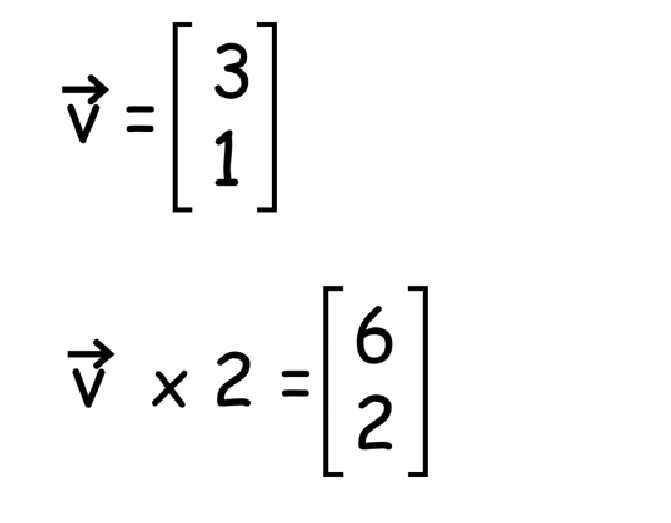
\includegraphics[width=0.5\linewidth,keepaspectratio]{vec2}
\end{center}

Multiply each element of the vector by the scalar
 
\end{frame}

%%%%%%%%%%%%%%%%%%%%%%%%%%%%%%%%%%%%%%%%%%%%%%%%%%%%%%%%%%%
 \begin{frame}[fragile] \frametitle{Scalar Vector Multiplication}

 \begin{lstlisting}
import numpy as np
import matplotlib.pyplot as plt
import math

v = np.array([2,1])

w = 2 * v
print(w)

# Plot w
origin = [0], [0]
plt.grid()
plt.ticklabel_format(style='sci', axis='both', scilimits=(0,0))
plt.quiver(*origin, *w, scale=10)
plt.show()
 \end{lstlisting}
 

 
\end{frame}

%%%%%%%%%%%%%%%%%%%%%%%%%%%%%%%%%%%%%%%%%%%%%%%%%%%%%%%%%%%
 \begin{frame}[fragile] \frametitle{Scalar Vector Multiplication}


\begin{center}
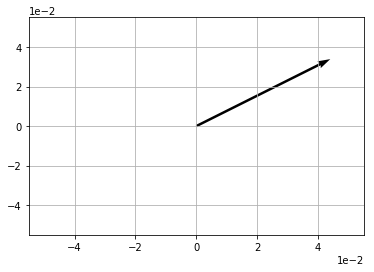
\includegraphics[width=0.5\linewidth,keepaspectratio]{vec5}
\end{center}

 
\end{frame}

%%%%%%%%%%%%%%%%%%%%%%%%%%%%%%%%%%%%%%%%%%%%%%%%%%%%%%%%%%%
 \begin{frame}[fragile] \frametitle{Scalar Vector Multiplication}

 $\vec{b} = \frac{\vec{v}}{2}$
 
 \begin{lstlisting}
b = v / 2
print(b)

# Plot b
origin = [0], [0]
plt.axis('equal')
plt.grid()
plt.ticklabel_format(style='sci', axis='both', scilimits=(0,0))
plt.quiver(*origin, *b, scale=10)
plt.show()
 \end{lstlisting}
 
[1.  0.5]
 
\end{frame}

%%%%%%%%%%%%%%%%%%%%%%%%%%%%%%%%%%%%%%%%%%%%%%%%%%%%%%%%%%%
 \begin{frame}[fragile] \frametitle{Scalar Vector Multiplication}


\begin{center}
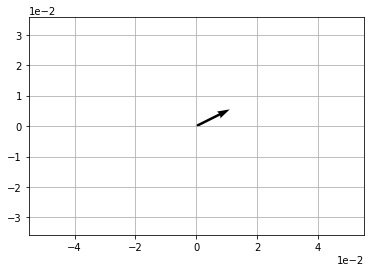
\includegraphics[width=0.5\linewidth,keepaspectratio]{vec6}
\end{center}

 
\end{frame}



%%%%%%%%%%%%%%%%%%%%%%%%%%%%%%%%%%%%%%%%%%%%%%%%%%%%%%%%%%%%%%%%%%%%%%%%%%%%%%%%%%
 \begin{frame}[fragile]\frametitle{}
\begin{center}
{\Large Dot Product}
\end{center}
\end{frame}



%%%%%%%%%%%%%%%%%%%%%%%%%%%%%%%%%%%%%%%%%%%%%%%%%%%%%%%%%%%
 \begin{frame}[fragile] \frametitle{Vector Vector Multiplication}
Dot Product
\begin{center}
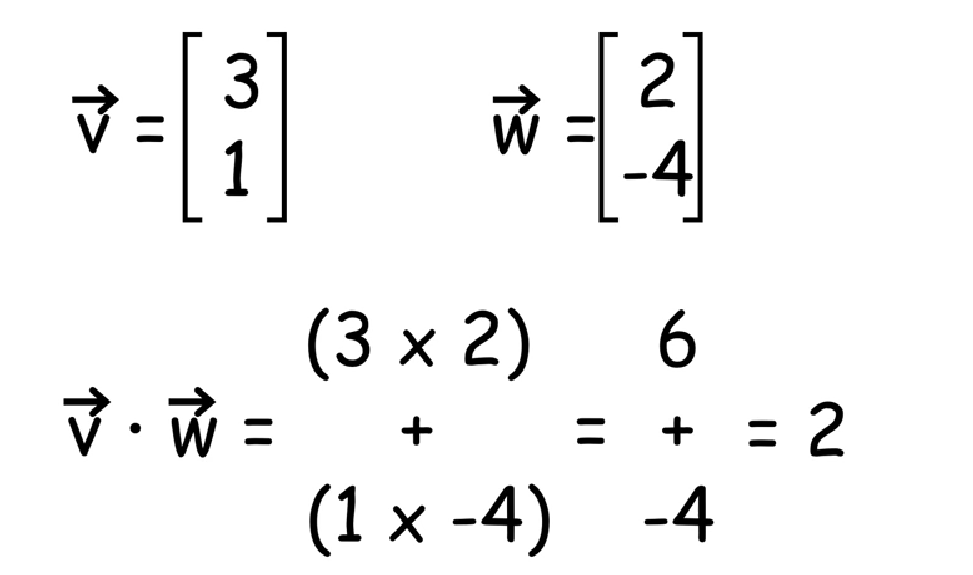
\includegraphics[width=0.5\linewidth,keepaspectratio]{vec3}
\end{center}

Multiply the corresponding elements of the vectors and add the results In this
case, 3 times 2 is 6, and 1 times -4 is -4; and adding these together
gives us our scalar result of 2. 

\end{frame}


%%%%%%%%%%%%%%%%%%%%%%%%%%%%%%%%%%%%%%%%%%%%%%%%%%%%%%%%%%%
 \begin{frame}[fragile] \frametitle{Vector Vector Multiplication}

$\vec{v} \cdot \vec{s} = (v_{1} \cdot s_{1}) + (v_{2} \cdot s_{2}) ... + \; (v_{n} \cdot s_{n})$
 
 \begin{lstlisting}
import numpy as np

v = np.array([2,1])
s = np.array([-3,2])
d = np.dot(v,s)
print (d)
 \end{lstlisting}
 
-4
 
\end{frame}


%%%%%%%%%%%%%%%%%%%%%%%%%%%%%%%%%%%%%%%%%%%%%%%%%%%%%%%%%%%
 \begin{frame}[fragile] \frametitle{Vector Vector Multiplication}

 \begin{itemize}
 
\item Another form: $\vec{v} \cdot \vec{s} = \|\vec{v} \|\|\vec{s}\| \cos (\theta)$ 

\item So for our vectors v (2,1) and s (-3,2), our calculation looks like this:

\item $\cos(\theta) = \frac{(2 \cdot-3) + (-3 \cdot 2)}{\sqrt{2^{2} + 1^{2}} \times \sqrt{-3^{2} + 2^{2}}}$

\item So $\cos(\theta) = -0.496138938357$

\item $\theta \approx 119.74$
\end{itemize}
 
\end{frame}

%%%%%%%%%%%%%%%%%%%%%%%%%%%%%%%%%%%%%%%%%%%%%%%%%%%%%%%%%%%
 \begin{frame}[fragile] \frametitle{Angle Between Two Vectors}

 \begin{itemize}
 
\item Suppose we have two vectors $\vec{v} = (v, 0)$ lying on X axis and $\vec{w}= (w_1,w_2)$
\item $w_1 = ||\vec{w}||cos\theta$, so $\theta = cos^{-1}(\frac{w_1}{||\vec{w}||})$
\item Now, dot product is given as $\vec{v}\cdot\vec{w} = v_1.w_1 + 0.w_2 = v_1.w_1$
\item Putting value of $w_1$, eqn becomes $= v_1.||\vec{w}||cos\theta = ||\vec{v}||||\vec{w}||cos\theta$
\item Therefore: $cos\theta = \frac{\vec{v}\cdot\vec{w}}{||\vec{v}||||\vec{w}||}$
\item Applicable to Higher Dimensions also!!
\end{itemize}
 
\end{frame}

%%%%%%%%%%%%%%%%%%%%%%%%%%%%%%%%%%%%%%%%%%%%%%%%%%%%%%%%%%%%%%%%%%%%%%%%%%%%%%%%%%
\begin{frame}[fragile] \frametitle{Definition}

Suppose that $\vec{u}, \vec{v}\in \mathbb R^n$.  We define the
 \textbf{inner product} or \textbf{dot procuct} or $\vec{u}$ and $\vec{v}$ as
 $$
 u\cdot v = u^tv=\sum_{i=1}^n u_i v_i.
 $$


\textbf{Example}
$$
 \left[ \begin{array}{r} 1\\2\\3 \end{array}\right] \cdot   \left[\begin{array}{r} -1\\-2\\1 \end{array}\right] =
 (1)(-1) + (2)(-2) + (3)(1) = -2.
 $$

\end{frame}

%%%%%%%%%%%%%%%%%%%%%%%%%%%%%%%%%%%%%%%%%%%%%%%%%%%%%%%%%%%%%%%%%%%%%%%%%%%%%%%%%%
\begin{frame}[fragile] \frametitle{Theorem}

Let $\vec{u}, \vec{v}, \vec{w} \in \mathbb R^n$ and let $c$  be a scalar.
Then 
\begin{itemize}
 \item $\vec{u}\cdot \vec{v} = \vec{v} \cdot \vec{u}$.
\item $(\vec{u} + \vec{v})\cdot \vec{w} = \vec{u}\cdot \vec{w}
+\vec{v}\cdot \vec{w}$.
\item $(c \vec{u})\cdot \vec{v}= c (\vec{u}\cdot \vec{v})$.
\item $\vec{u} \cdot \vec{u} \geq 0$ and $\vec{u}\cdot \vec{u} = 0$ 
if and only if $\vec{u} = \vec{0}$.
\item $(c_1 \vec{u}_1 +\dots + c_p \vec{u}_p)\cdot \vec{w} = c_1\vec{u}_1\cdot \vec{w}
+c_p\vec{u}_p\cdot \vec{w}$.
\end{itemize}
 

\textbf{Definition}[Length]
The {\em length} (or {\em norm})  of $\vec{v}$ is the non-negative scalar $\|\vec{v}\|$ 
defined by 
\[
 \| \vec{v} \| = \sqrt{\vec{v} \cdot \vec{v}} =
\sqrt{v_1^2 + v_2^2 +\dots + v_n^2} \ \text{ and } \ \|\vec{v} \|^2 = 
\vec{v}\cdot \vec{v}.
 \]

\end{frame}


%%%%%%%%%%%%%%%%%%%%%%%%%%%%%%%%%%%%%%%%%%%%%%%%%%%%%%%%%%%%%%%%%%%%%%%%%%%%%%%%%%
\begin{frame}[fragile] \frametitle{Note}
 This definition is chosen so that the Pythagorean theorem holds (that is, in two 
dimensions the length $c$ of the vector which is the hypotenuse of a right triangle 
with horizontal length $a$ and vertical height $b$ satisfies $a^2 + b^2 = c^2$. 
 

\textbf{Facts}
\begin{itemize}
 \item For any scalar $c$, $\| c\vec{v}\| = |c| \ \|\vec{v}\|$.  
 \item A vector of length 1 is called a \textbf{unit vector}.  
 \item  If $\vec{v}\neq \vec{0}$ then $\frac{1}{\| \vec{v} \|} \vec{v}$ 
is a unit vector and is in the same direction as $\vec{v}$.   
 \item  The above process is called normalizing. 
\end{itemize}

\end{frame}


%%%%%%%%%%%%%%%%%%%%%%%%%%%%%%%%%%%%%%%%%%%%%%%%%%%%%%%%%%%%%%%%%%%%%%%%%%%%%%%%%%
\begin{frame}[fragile] \frametitle{Example}
 Find a unit vector which is in the same direction as $\vec{v} =
\left[ \begin{array}{rrrr} 1 \\ 1 \\ 2 \end{array} \right]$.
 

\textbf{Definition}
For $\vec{u}$ and $\vec{v}$ in $\mathbb R^n$, the {\em distance between $\vec{u}$
and $\vec{v}$}, written as $\text{dist}(\vec{u},\vec{v})$ is the length
of the vector $\vec{u}-\vec{v}$.  That is,
\[
 \text{dist}(\vec{u},\vec{v})  = \| \vec{u} - \vec{v} \|.
\]
  

\textbf{Example}
 Compute the distance 
$\text{dist}\left[\left[ \begin{array}{rrrr}7 \\ 2 \end{array} \right],\left[ \begin{array}{rrrr} 4 \\ 3 \end{array} \right]\right]$.

\end{frame}

%%%%%%%%%%%%%%%%%%%%%%%%%%%%%%%%%%%%%%%%%%%%%%%%%%%%%%%%%%%%%%%%%%%%%%%%%%%%%%%%%%
\begin{frame}[fragile] \frametitle{Orthogonal Vectors}
 Two vectors in $\mathbb R^n$ are {\em orthogonal} if and only if $\vec{u}\cdot\vec{v}=0$.

\begin{itemize}
\item Angle between two vectors is 0, meaning $cos\theta = 0$ meaning $\theta = 90$ degrees.
\item In 2D, there will be two such orthogonal (perpendicular) vectors to a given vector.
\item if the given vector is 3D, there will be infinite such orthogonal vectors, but all will lie in a single plane.
\item In higher dimensions, the orthogonal entity is called as a Hyperplane, all passing through base of the vector.
\item Hyperplane separates space into 2  halves.
\end{itemize}

\end{frame}

%%%%%%%%%%%%%%%%%%%%%%%%%%%%%%%%%%%%%%%%%%%%%%%%%%%%%%%%%%%%%%%%%%%%%%%%%%%%%%%%%%
\begin{frame}[fragile] \frametitle{Orthogonal Vectors}
 Two vectors in $\mathbb R^n$ are {\em orthogonal} if and only if $\vec{u}\cdot\vec{v}=0$.
  

\textbf{Note}
\begin{eqnarray*}
 \| \vec{u} -\vec{v}\|^2 & =  & (\vec{u}-\vec{v})\cdot(\vec{u}- \vec{v})\\
& = & \vec{u}\cdot \vec{u} - \vec{u} \cdot \vec{v} 
      - \vec{v} \cdot \vec{u} + \vec{v}\vec{v} \\
& = & \| \vec{u} \|^2 + \| \vec{v}\|^2 - 2 \vec{u}\cdot\vec{v}
\end{eqnarray*}


\textbf{Theorem}[Pythagorus]
 $||\vec{u} - \vec{v}||^2 = ||\vec{u}||^2 + ||\vec{v}||^2$ if and only if $\vec{u}$ and $\vec{v}$ are orthogonal.


\end{frame}

%%%%%%%%%%%%%%%%%%%%%%%%%%%%%%%%%%%%%%%%%%%%%%%%%%%%%%%%%%%%%%%%%%%%%%%%%%%%%%%%%%
\begin{frame}[fragile] \frametitle{Definition}

Suppose that $W\le \mathbb R^n$.
\begin{itemize}
  \item  If for all $\vec{w}\in W$, $\vec{z}\cdot\vec{w}=0$,l then we say that $\vec{z}$ is orthogonal to $W$ and write $z\perp W$.
  \item We define the orthogonal compliment of $W$ as $W^{\perp}=\{\vec{z}\in \mathbb R^n \vec{z}\perp W\}$.
\end{itemize}
  

\textbf{Example}
 Suppose that $W=\mbox{Span} \left(\left(\begin{array}{r}1\\0\\0\end{array}\right), \left(\begin{array}{r} 0\\1\\0\end{array}\right)  \right)$.  \\
 Describe $W^{\perp}$.

\end{frame}


%%%%%%%%%%%%%%%%%%%%%%%%%%%%%%%%%%%%%%%%%%%%%%%%%%%%%%%%%%%%%%%%%%%%%%%%%%%%%%%%%%
\begin{frame}[fragile] \frametitle{Fact}
\begin{itemize}
  \item $\vec{x}\in W^{\perp}$ if and only if $\vec{x}\perp \vec{w}$ for all $\vec{w}$ in a spanning set for $W$.
  \item  $W^{\perp}\le \mathbb R^n$.
\end{itemize}
  

\textbf{Theorem}
 Suppose that $A$ is an $n\times n$ matrix.
\begin{itemize}
  \item $(\mbox{Row}(A))^{\perp} = \mbox{Nul}(A)$.
  \item $(\mbox{Col}(A))^{\perp}=\mbox{Nul}(A^t)$.
\end{itemize}

\end{frame}


%%%%%%%%%%%%%%%%%%%%%%%%%%%%%%%%%%%%%%%%%%%%%%%%%%%%%%%%%%%%%%%%%%%%%%%%%%%%%%%%%%
\begin{frame}[fragile] \frametitle{Note}
 In two or three dimensions, the projection of $\vec{v}$ onto $\vec{u}$
has length $\| \vec{v} \| \cos \theta$, where $\theta$ is the angle between
the vectors.  Hence
\[
 \| \vec{v} \| \cos \theta = c \| \vec{u} \|
\]
so that 
\[
 \vec{u}\cdot\vec{v} = \| \vec{u} \| \| \vec{v} \| \cos \theta.
\]
In higher dimensions than three we use this to {\em define} the angle between two vectors.

\end{frame}

%%%%%%%%%%%%%%%%%%%%%%%%%%%%%%%%%%%%%%%%%%%%%%%%%%%%%%%%%%%%%%%%%%%%%%%%%%%%%%%%%%
\begin{frame}[fragile] \frametitle{Definition}
 Two vectors in $\mathbb R^n$ are {\em orthogonal} if and only if $\vec{u}\cdot\vec{v}=0$.
  

\textbf{Note}
\begin{eqnarray*}
 \| \vec{u} -\vec{v}\|^2 & =  & (\vec{u}-\vec{v})\cdot(\vec{u}- \vec{v})\\
& = & \vec{u}\cdot \vec{u} - \vec{u} \cdot \vec{v} 
      - \vec{v} \cdot \vec{u} + \vec{v}\vec{v} \\
& = & \| \vec{u} \|^2 + \| \vec{v}\|^2 - 2 \vec{u}\cdot\vec{v}
\end{eqnarray*}
 

\textbf{Theorem}[Pythagorus]
 $||\vec{u} - \vec{v}||^2 = ||\vec{u}||^2 + ||\vec{v}||^2$ if and only if $\vec{u}$ and $\vec{v}$ are orthogonal.


\end{frame}



\newcommand{\R}{\mathbb{R}}

\newcommand{\norm}[1]{\lVert#1\rVert} % norm

\newcommand{\avg}[1]{\left< #1 \right>} % average

\newcommand{\sabs}[1]{\left| #1 \right|} % smaller absolute value
\newcommand{\abs}[1]{\bigl| #1 \bigr|} % absolute value



%%%%%%%%%%%%%%%%%%%%%%%%%%%%%%%%%%%%%%%%%%%%%%%%%%%%%%%%%%%%%%%%%%%%%%%%%%%%%%%%%%
\begin{frame}[fragile] \frametitle{Inner products}

\textbf{Definition}: An {\em inner product} on a real vector space $V$ is an operation (function) that assigns to each pair of vectors $(\vec{u}, \vec{v})$ in $V$ a \textbf{scalar} $\avg{ \vec{u}, \vec{v} }$ satisfying the following axioms:

\begin{itemize}

\item  $\avg{ \vec{u}, \vec{v} } =  \avg{ \vec{v}, \vec{u} } $   \ (Symmetry)

\item   $\avg{ \vec{u} + \vec{v}, \vec{w} }   =  \avg{ \vec{u}, \vec{w} } +  \avg{ \vec{v}, \vec{w} }$  \ (Additivity)

\item  $\avg{ k \, \vec{u}, \vec{v} }  = k  \, \avg{ \vec{u}, \vec{v} }$ \ (Homogeneity)

\item  $\avg{ \vec{v}, \vec{v} } \, \ge 0$  \ and  $\avg{ \vec{v}, \vec{v} } = 0$ iff $\vec{v} = \vec{0}$ \ (Positivity)


\end{itemize}





\textbf{Theorem} (basic properties): Given vectors $\vec{u}, \vec{v}, \vec{w}$ in an inner product space $V$, and a scalar $k$, the following properties hold:

\begin{itemize}

\item $\avg{ \vec{\rm{o}}, \vec{v} } = \avg{ \vec{v}, \vec{\rm{o}} }  = 0$

\item $\avg{ \vec{u} - \vec{v}, \vec{w} }   =  \avg{ \vec{u}, \vec{w} } -  \avg{ \vec{v}, \vec{w} }$

\item $\avg{ \vec{u}, \vec{v} + \vec{w} }   =  \avg{ \vec{u}, \vec{v} } +  \avg{ \vec{u}, \vec{w} }$

\item $\avg{ \vec{u}, \vec{v} - \vec{w} }   =  \avg{ \vec{u}, \vec{v} }  -  \avg{ \vec{u}, \vec{w} }$

\item  $\avg{ \vec{u}, k \vec{ v} }  = k  \, \avg{ \vec{u}, \vec{v} }$

\end{itemize}

\end{frame}


%%%%%%%%%%%%%%%%%%%%%%%%%%%%%%%%%%%%%%%%%%%%%%%%%%%%%%%%%%%%%%%%%%%%%%%%%%%%%%%%%%
 \begin{frame}[fragile]\frametitle{Norm and distance in an inner product space}

\textbf{Definition}: If $V$ is a real inner product space then we define

\begin{itemize}

\item The norm (or length) of $\vec{v}$:
$$\norm{\vec{v}} = \sqrt{ \avg{ \vec{v}, \vec{v} } } $$

\item The distance between $\vec{u}$ and $\vec{v}$:
$$ d (\vec{u}, \vec{v}) = \norm{ \vec{u} - \vec{v}} =  \sqrt{ \avg{ \vec{u} - \vec{v}, \vec{u} - \vec{v} } } $$

\end{itemize}



\textbf{Theorem} (basic properties): Given vectors $\vec{u}, \vec{v}$ in an inner product space $V$, and a scalar $k$, the following properties hold:

\begin{itemize}

\item $\norm{\vec{v}} \ge 0$ \ and \ $\norm{\vec{v}} = 0$ iff $\vec{v} = \vec{0}$.

\item $\norm{ k \vec{v}} = |k| \, \norm{\vec{v}}$

\item $d (\vec{u}, \vec{v}) = d (\vec{v}, \vec{u}) $

\item $d (\vec{u}, \vec{v} ) \ge 0$ \ and \ $d (\vec{u}, \vec{v}) = 0$ iff $\vec{u} = \vec{v}$.


\end{itemize}

\end{frame}


%%%%%%%%%%%%%%%%%%%%%%%%%%%%%%%%%%%%%%%%%%%%%%%%%%%%%%%%%%%%%%%%%%%%%%%%%%%%%%%%%%
 \begin{frame}[fragile]\frametitle{Angle between vectors}

\textbf{Theorem} (Cauchy-Schwarz): If $u$ and $v$ are vectors in an inner vector space, then
$$\abs{ \avg{u, v} } \le \norm{u} \, \norm{v} $$




\textbf{Definition}: The angle between two vectors  $u$ and $v$ in an inner vector space is defined as
$$\theta = \cos^{-1} \, \frac{\avg{u,v}}{\norm{u} \, \norm{v}}  $$





\textbf{Theorem} (the triangle inequality):  If $u, v$ and $w$ are vectors in an inner vector space, then
\begin{itemize}
\item $\norm{u + v} \le \norm{u} + \norm{v}$

\item $d (u, v) \le d (u, w) + d (w, v)$
\end{itemize}

\end{frame}


%%%%%%%%%%%%%%%%%%%%%%%%%%%%%%%%%%%%%%%%%%%%%%%%%%%%%%%%%%%
 \begin{frame}[fragile] \frametitle{Orthogonality}
\textbf{Definition}:  Two vectors  $u$ and $v$ in an inner vector space are called {\em orthogonal} if $\avg{u, v} = 0$.
\smallskip
Clearly $u \perp v$ iff the angle between them is $\theta = \frac{\pi}{2}$.
\textbf{Theorem} (the Pythagorean theorem):  If $u$ and $v$ are \textbf{orthogonal} vectors in an inner vector space, then
$$\norm{u + v}^2 = \norm{u}^2 + \norm{v}^2$$
\end{frame}

%%%%%%%%%%%%%%%%%%%%%%%%%%%%%%%%%%%%%%%%%%%%%%%%%%%%%%%%%%%%%%%%%%%%%%%%%%%%%%%%%%
\begin{frame}[fragile]\frametitle{Orthogonality}
\textbf{Definition}:  Let $W$ be a subspace of an inner product space $V$. 
The set of vectors in $V$ which are orthogonal to \textbf{every} vector in $W$ is called the {\em orthogonal complement} of $W$ and it is denoted by $W^\perp$.
\textbf{Theorem}: The orthogonal complement has the following properties:
\begin{itemize}
\item $W^\perp$ is a subspace of $V$.
\item $W \cap W^\perp = \{ \vec{\rm{o}} \}$.
\item If $V$ has finite dimension then $(W^\perp)^\perp = W$.
\end{itemize}
\end{frame}

%%%%%%%%%%%%%%%%%%%%%%%%%%%%%%%%%%%%%%%%%%%%%%%%%%%%%%%%%%%%%%%%%%%%%%%%%%%%%%%%%%
 \begin{frame}[fragile]\frametitle{Orthogonal sets, orthonormal sets}
Let $(V, \avg{ \ })$ be an inner product space and let $S$ be a set of vectors in $V$.
\textbf{Definition}: The set $S$  is called {\em orthogonal} if any two vectors in $S$  are orthogonal.
The set $S$ is called {\em orthonormal} if it is orthogonal and any vector in $S$ has norm $1$.
\textbf{Theorem}: Every orthogonal set of nonzero vectors is linearly independent.

\end{frame}

%%%%%%%%%%%%%%%%%%%%%%%%%%%%%%%%%%%%%%%%%%%%%%%%%%%%%%%%%%%%%%%%%%%%%%%%%%%%%%%%%%
 \begin{frame}[fragile]
\frametitle{Orthogonal sets, orthonormal sets}
\textbf{Definition}: A set of vectors $S$  is called an {\em orthogonal} basis (OGB) for $V$ if $S$ is a basis and an orthogonal set (that is, $S$ is a basis where all vectors are perpendicular).

A set of vectors $S$  is called an {\em orthonormal} basis (ONB) for $V$ if $S$ is a basis and an orthonormal set (that is, $S$ is a basis where all vectors are perpendicular and have norm $1$).
\end{frame}

%%%%%%%%%%%%%%%%%%%%%%%%%%%%%%%%%%%%%%%%%%%%%%%%%%%%%%%%%%%%%%%%%%%%%%%%%%%%%%%%%%
 \begin{frame}[fragile]\frametitle{Orthogonal sets, orthonormal sets}

Let $(V, \avg{ \ })$ be an inner product space.

\textbf{Theorem}:  If $S = \{ v_1, v_2, \ldots, v_n \}$ is an orthogonal basis in $V$ and $u$ is any vector in $V$, then
$$u = \frac{\avg{u, v_1}}{\norm{v_1}^2} \, v_1 + \frac{\avg{u, v_2}}{\norm{v_2}^2} \, v_2 + \ldots + \frac{\avg{u, v_n}}{\norm{v_n}^2} \, v_n$$

If $S = \{ v_1, v_2, \ldots, v_n \}$ is an orthonormal basis in $V$ and $u$ is any vector in $V$, then
$$u = \avg{u, v_1} \, v_1 + \avg{u, v_2} \, v_2  + \ldots + \avg{u, v_n} \, v_n$$ 

\end{frame}


%%%%%%%%%%%%%%%%%%%%%%%%%%%%%%%%%%%%%%%%%%%%%%%%%%%%%%%%%%%%%%%%%%%%%%%%%%%%%%%%%%
 \begin{frame}[fragile]\frametitle{}
\begin{center}
{\Large Cross Product}
\end{center}
\end{frame}


%%%%%%%%%%%%%%%%%%%%%%%%%%%%%%%%%%%%%%%%%%%%%%%%%%%%%%%%%%%
 \begin{frame}[fragile] \frametitle{Vector Vector Multiplication}
Cross Product (for 3D vectors)
\begin{center}
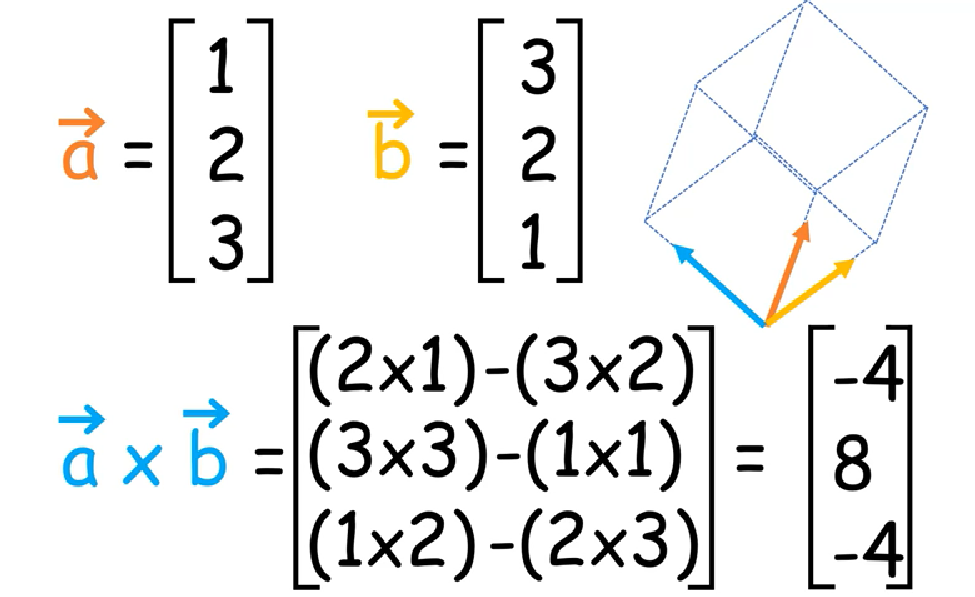
\includegraphics[width=0.5\linewidth,keepaspectratio]{vec4}
\end{center}
Skipping the current row and column, calculate determinant value of remaining sub matrix for that position.
\end{frame}


%%%%%%%%%%%%%%%%%%%%%%%%%%%%%%%%%%%%%%%%%%%%%%%%%%%%%%%%%%%
 \begin{frame}[fragile] \frametitle{Vector Vector Multiplication}
Cross Product
 \begin{itemize}
 
\item $\vec{p} = \begin{bmatrix}2 \\ 3 \\ 1 \end{bmatrix}\;\; \vec{q} = \begin{bmatrix}1 \\ 2 \\ -2 \end{bmatrix}$
\item \begin{align}r_{1} = p_{2}q_{3} - p_{3}q_{2} \\ r_{2} = p_{3}q_{1} - p_{1}q_{3} \\ r_{3} = p_{1}q_{2} - p_{2}q_{1} \end{align}
\item $\vec{r} = \vec{p} \times \vec{q} = \begin{bmatrix}(3 \cdot -2) - (1 \cdot 2) \\ (1 \cdot 1) - (2 \cdot -2) \\ (2 \cdot 2) - (3 \cdot 1) \end{bmatrix} = \begin{bmatrix}-6 - 2 \\ 1 - -4 \\ 4 - 3 \end{bmatrix} = \begin{bmatrix}-8 \\ 5 \\ 1 \end{bmatrix}$
\end{itemize}
 
\end{frame}


%%%%%%%%%%%%%%%%%%%%%%%%%%%%%%%%%%%%%%%%%%%%%%%%%%%%%%%%%%%
 \begin{frame}[fragile] \frametitle{Vector Vector Multiplication}

Cross Product
 
 \begin{lstlisting}
import numpy as np

p = np.array([2,3,1])
q = np.array([1,2,-2])
r = np.cross(p,q)
print (r)
 \end{lstlisting}
 
[-8  5  1]
\end{frame}

%%%%%%%%%%%%%%%%%%%%%%%%%%%%%%%%%%%%%%%%%%%%%%%%%%%%%%%%%%%%%%%%%%%%%%%%%%%%%%%%%%
 \begin{frame}[fragile]\frametitle{}
\begin{center}
{\Large Linear Combinations}
\end{center}
\end{frame}




%%%%%%%%%%%%%%%%%%%%%%%%%%%%%%%%%%%%%%%%%%%%%%%%%%%%%%%%%%%
  \begin{frame}[fragile]\frametitle{Linear Combinations}
\textbf{Definition}
Let $p$ be a positive integer. Given vectors $\vec{u}_1, \vec{u}_2, \dots \vec{u}_p$
in $\mathbb R^n$, and $c_1, c_2, \dots c_p$ in $\mathbb R$, the vector
\[
 \vec{u} = c_1 \vec{u}_1 + c_2 \vec{u}_2 + \dots c_p\vec{u}_p
\]
is called a linear combination of the vectors $\vec{u}_1, \dots \vec{u}_p$ with
weights $c_1, \dots c_p$.

\end{frame}

%%%%%%%%%%%%%%%%%%%%%%%%%%%%%%%%%%%%%%%%%%%%%%%%%%%%%%%%%%%
  \begin{frame}[fragile]
\textbf{Example}
\[
 2\left[\begin{array}{r}1 \\-2 \\ 7  \end{array}\right]\ 
 + \ 3\left[\begin{array}{r} 1 \\ 1 \\ 1 \end{array}\right] \ 
 + \ -2\left[\begin{array}{r}2 \\ 3 \\ -8  \end{array}\right]
 = \left[\begin{array}{r}\qquad  \\ \qquad \\ \qquad \end{array}\right] \]     
is a linear combination of $ \left[\begin{array}{r}1 \\-2 \\ 7  \end{array}\right],$ $\left[\begin{array}{r} 1 \\ 1 \\ 1 \end{array}\right]$ and $\left[\begin{array}{r}2 \\ 3 \\ -8  \end{array}\right]$ with weights $2,3 ,-2$.


\textbf{Geometry} 
Let $\vec{u} = \left[\begin{array}{r} 1 \\ 1 \end{array}\right]$ and 
$\vec{v} = \left[\begin{array}{r} 1 \\ -1 \end{array}\right]$.  Show all
linear combinations of $\vec{u}$ and $\vec{v}$ on a graph.

\end{frame}

%%%%%%%%%%%%%%%%%%%%%%%%%%%%%%%%%%%%%%%%%%%%%%%%%%%%%%%%%%%
  \begin{frame}[fragile]
\textbf{Exercise}
let 
$\vec{u}_1 = \left[\begin{array}{r} 1 \\ 2 \\ 5 \end{array}\right]$
$\vec{u}_2 = \left[\begin{array}{r} 2 \\ 1 \\ 3 \end{array}\right]$ and 
$\vec{b} = \left[\begin{array}{r} -4 \\ 1 \\ 1 \end{array}\right]$
Is $\vec{b}$ a linear combination of $\vec{u}_1$ and $\vec{u}_2$

\end{frame}

%%%%%%%%%%%%%%%%%%%%%%%%%%%%%%%%%%%%%%%%%%%%%%%%%%%%%%%%%%%
  \begin{frame}[fragile]\frametitle{Vector Equations}
\textbf{Facts}
A vector equation 
\[
 x_1 \vec{v}_1  + x_2 \vec{v}_2 + \dots + x_n \vec{v}_n =\vec{b}
\]
has the same solution set as the system of equations whose augmented matrix is 
\[
 \left[\begin{array}{ccccc}
  | & | & \dots & | & | \\
  \vec{v}_1 & \vec{v}_2 & \dots & \vec{v}_n & \vec{b} \\
  | & | & \dots & | & | \\
 \end{array}\right]
\]
In particular, $\vec{b}$ is a linear combination of $\vec{v}_1, \dots \vec{v}_n$
if and only if the system of linear equations is consistent.

\end{frame}

%%%%%%%%%%%%%%%%%%%%%%%%%%%%%%%%%%%%%%%%%%%%%%%%%%%%%%%%%%%
  \begin{frame}[fragile]
\textbf{Definition}
 Suppose $\vec{v}_1, \vec{v}_2, \dots \vec{v}_p \in \mathbb R^n$.
 We define 
 \[
  \mbox{Span}(\vec{v}_1, \vec{v}_2, \dots ,\vec{v}_p) =
 \left\{
 c_1 \vec{v}_1 + c_2 \vec{v}_2 + \dots c_p \vec{v}_p: c_1, c_2, \dots , c_p \in \mathbb R 
 \right\}
 \]    
 That is, Span$(\vec{v}_1, \dots , \vec{v}_p)$ is the set of all linear combinations
of $\vec{v}_1, \dots , \vec{v}_p$.

\end{frame}

%%%%%%%%%%%%%%%%%%%%%%%%%%%%%%%%%%%%%%%%%%%%%%%%%%%%%%%%%%%
  \begin{frame}[fragile]\frametitle{Geometry}
\textbf{Note}
\begin{itemize}
\item The span of $\vec{0}$ in $\mathbb R^2$ or $\mathbb R^3$ is the single point $\vec{0}$.
\item The span of a single non-zero vector in $\mathbb R^2$ or $\mathbb R^3$ is a line through $\vec{0}$.
\item The span of two non-zero vectors in $\mathbb R^3$ is either a plane through $\vec{0}$ or, if one
vector is a scalar multiple of the other, a line through $\vec{0}$.
\end{itemize}


\textbf{Exercise}
Let $\vec{v}_1 = \left[\begin{array}{r}1 \\ 1 \\ 2 \end{array}\right]$, 
$\vec{v}_2 = \left[\begin{array}{r} 2 \\ 5 \\ -3 \end{array}\right]$ and 
$\vec{b} = \left[\begin{array}{r} -9 \\ -30 \\ 31 \end{array}\right]$.
Span$(\vec{v}_1,\vec{v}_2)$ is a plane in $\mathbb R^3$  Is $\vec{b}$ in that plane?

\end{frame}
